\documentclass[aspectratio=169]{beamer}
%\setbeameroption{show notes}

\usepackage{beamer_pre}


\title{Thesis meeting 2024/03/27}
\author{Albert R. S. Garde}
\date{\today}
	

\begin{document}

\frame{
	\maketitle
}

\begin{frame}[fragile=singleslide]
	\frametitle{Progress since last meeting}
    \begin{itemize}
        \item Solved the critical issue.
        \begin{itemize}
            \item Took me a month of very inefficient work to get to a point where I could start debugging.
            \item Debugged it within 30 minutes.
        \end{itemize}
        \item Ran statistics again.
        \item Succesfully integrated my reimplementation of NeuronModel, but it performed far worse
    \end{itemize}
\end{frame}
\begin{frame}[fragile=singleslide]
    \frametitle{Results}
    \begin{itemize}
        \item Statistics are similar to before, but now there are almost no NaNs.
        \item N2G models of SAE features generally have better performance, but have a weird distribution.
        \item No significant difference on recall, \emph{very} significant difference on precision (and F1).
    \end{itemize}
    \begin{center}
        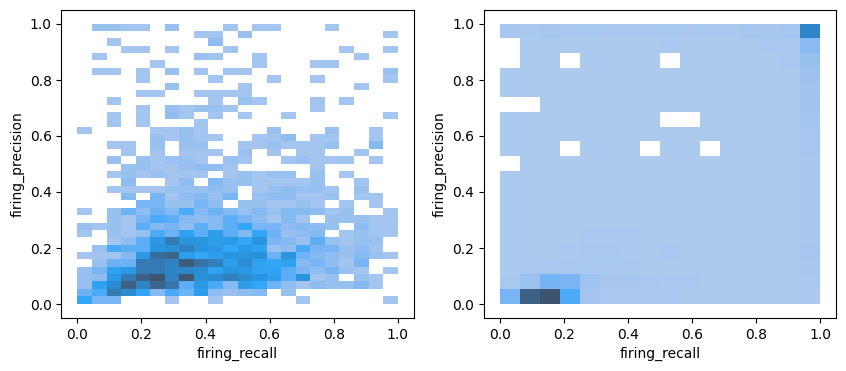
\includegraphics[width=\linewidth]{images/heatmap.png}
    \end{center}
\end{frame}
\begin{frame}[fragile=singleslide]
    \frametitle{Results}
    \begin{itemize}
        \item Statistics are similar to before, but now there are almost no NaNs.
        \item N2G models of SAE features generally have better performance, but have a weird distribution.
        \item No significant difference on recall, \emph{very} significant difference on precision (and F1).
    \end{itemize}
    \begin{center}
        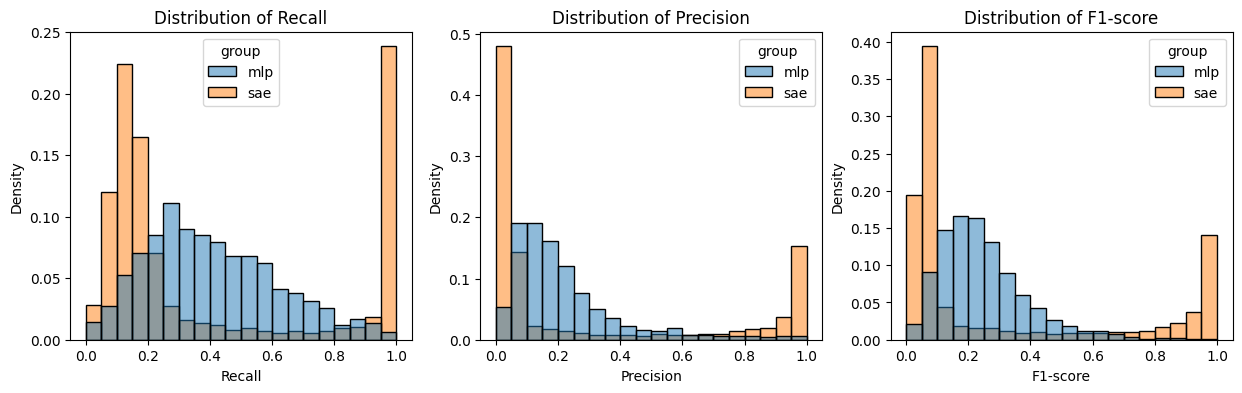
\includegraphics[width=\linewidth]{images/histogram.png}
    \end{center}
\end{frame}
\begin{frame}[fragile=singleslide]
    \frametitle{Plan for the next weeks}
    \begin{itemize}
        \item Get statistics on how well the models predict specific activation instead of just whether the feature "activates".
        \item Run on other SAEs. Especially SAEs of models with more than 1 layer would be very interesting.
        \item Write draft of methodology section.
        \item Keep working on the NeuronModel implementation.
    \end{itemize}
\end{frame}
\begin{frame}[fragile=singleslide]
    \frametitle{Topics for meeting}
    \begin{itemize}
        \item What do these results tell us?
        \item What would be worth investigating?
        \begin{itemize}
            \item Comparison with other measures of interpretability?
            \item 
        \end{itemize}
        \item How far are we from having a thesis worthy result?
    \end{itemize}
\end{frame}

\end{document}